 Define Article %%%%%
\documentclass[addpoints]{exam}
%%%%%%%%%%%%%%%%%%%%%

 Using Packages %%%%%
\usepackage{geometry}
\usepackage{graphicx}
\usepackage{amssymb}
\usepackage{amsmath}
\usepackage{amsthm}
\usepackage{empheq}
\usepackage{mdframed}
\usepackage{booktabs}
\usepackage{lipsum}
\usepackage{graphicx}
\usepackage{color}
\usepackage{psfrag}
\usepackage{pgfplots}
\usepackage{bm}
\usepackage{listings}
\usepackage{xcolor}
\usepackage{verbatim}

\definecolor{codegreen}{rgb}{0,0.6,0}
\definecolor{codegray}{rgb}{0.5,0.5,0.5}
\definecolor{codepurple}{rgb}{0.58,0,0.82}
\definecolor{backcolour}{rgb}{0.95,0.95,0.92}

\lstdefinestyle{mystyle}{
    backgroundcolor=\color{backcolour},   
    commentstyle=\color{codegreen},
    keywordstyle=\color{magenta},
    numberstyle=\tiny\color{codegray},
    stringstyle=\color{codepurple},
    basicstyle=\ttfamily\footnotesize,
    breakatwhitespace=false,         
    breaklines=true,                 
    captionpos=b,                    
    keepspaces=true,                 
    numbers=left,                    
    numbersep=5pt,                  
    showspaces=false,                
    showstringspaces=false,
    showtabs=false,                  
    tabsize=2
}

\lstset{style=mystyle}

%%%%%%%%%%%%%%%%%%%%%

% Other Settings

%%%%%%%%%%%%%%%%%%%%%%%%%% Page Setting %%%%%%%%%%
\geometry{a4paper}
\printanswers

%%%%%%%%%%%%%%%%%%%%%%%%%% Define some useful colors %%%%%%%%%%%%%%%%%%%%%%%%%%
\definecolor{ocre}{RGB}{243,102,25}
\definecolor{mygray}{RGB}{243,243,244}
\definecolor{deepGreen}{RGB}{26,111,0}
\definecolor{shallowGreen}{RGB}{235,255,255}
\definecolor{deepBlue}{RGB}{61,124,222}
\definecolor{shallowBlue}{RGB}{235,249,255}
%%%%%%%%%%%%%%%%%%%%%

%%%%%%%%%%%%%%%%%%%%%%%%%% Define an orangebox command %%%%%%%%%%%%%%%%%%%%%%%%
\newcommand\orangebox[1]{\fcolorbox{ocre}{mygray}{\hspace{1em}#1\hspace{1em}}}
%%%%%%%%%%%%%%%%%%%%%

%%%%%%%%%%%%%%%%%%%%%%%%%%%% English Environments 
\newtheoremstyle{mytheoremstyle}{3pt}{3pt}{\normalfont}{0cm}{\rmfamily\bfseries}{}{1em}{{\color{black}\thmname{#1}~\thmnumber{#2}}\thmnote{\,--\,#3}}
\newtheoremstyle{myproblemstyle}{3pt}{3pt}{\normalfont}{0cm}{\rmfamily\bfseries}{}{1em}{{\color{black}\thmname{#1}~\thmnumber{#2}}\thmnote{\,--\,#3}}
\theoremstyle{mytheoremstyle}
\newmdtheoremenv[linewidth=1pt,backgroundcolor=shallowGreen,linecolor=deepGreen,leftmargin=0pt,innerleftmargin=20pt,innerrightmargin=20pt,]{theorem}{Theorem}[section]
\theoremstyle{mytheoremstyle}
\newmdtheoremenv[linewidth=1pt,backgroundcolor=shallowBlue,linecolor=deepBlue,leftmargin=0pt,innerleftmargin=20pt,innerrightmargin=20pt,]{definition}{Definition}[section]
\theoremstyle{myproblemstyle}
\newmdtheoremenv[linecolor=black,leftmargin=0pt,innerleftmargin=10pt,innerrightmargin=10pt,]{problem}{Problem}[section]
%%%%%%%%%%%%%%%%%%%%%

%% Plotting Settings 
\usepgfplotslibrary{colorbrewer}
\pgfplotsset{width=8cm,compat=1.9}
%%%%%%%%%%%%%%%%%%%%%

%% Title & Author %%%
\title{Statistical Inference Homework 1}
\author{Muhammad Meesum Ali Qazalbash}
%%%%%%%%%%%%%%%%%%%%%

\begin{document}
\maketitle

\begin{questions}
	\question Suppose that \(X\) is a discrete random variable with probability mass function given by
	\begin{align*}
		\operatorname{P}(X=0) & =\frac{2}{3}\theta     \\
		\operatorname{P}(X=1) & =\frac{1}{3}\theta     \\
		\operatorname{P}(X=2) & =\frac{2}{3}(1-\theta) \\
		\operatorname{P}(X=3) & =\frac{1}{3}(1-\theta)
	\end{align*}
	where \(0\leq\theta\leq1\) is parameter. The following 10 independents obeservations were taken from such a distribution: \((3, 0, 2, 1, 3, 2, 1, 0, 2, 1)\).

	\begin{parts}
		\part Find the maximum likelihood estimator of \(\theta\).

		\begin{solution}
			\begin{align*}
				\operatorname{lik}(\theta)                 & = f\left(x_{1},x_{2},\cdots,x_{n}|\theta\right)                                                               \\
				                                           & = \prod_{i=1}^n f(x_i|\theta)                                                                                 \\
				\implies \log{\operatorname{lik}(\theta)}  & = \sum_{i=1}^n \log{f(x_i|\theta)}                                                                            \\
				l(\theta)                                  & = \sum_{i=1}^n \log{\operatorname{P}(X=x_{i})}                                                                \\
				                                           & = 2\log{\frac{2}{3}\theta}+3\log{\frac{1}{3}\theta}+3\log{\frac{2}{3}(1-\theta)}+2\log{\frac{1}{3}(1-\theta)} \\
				                                           & = 5\log{\frac{2}{9}}+5\log{(\theta-\theta^{2})}                                                               \\
				\implies \frac{\partial l}{\partial\theta} & = \frac{5(1-2\theta)}{\theta-\theta^{2}} = 0                                                                  \\
				\implies \hat{\theta}                      & = \frac{1}{2}
			\end{align*}
		\end{solution}

		\newpage

		\part Prove that \(\displaystyle l'(\theta)=\frac{5-10\theta}{\theta(1-\theta)}\) and \(\displaystyle l''(\theta)=-\frac{5(2\theta^{2}-2\theta+1)}{\left[\theta(1-\theta)\right]^{2}}\).

		\begin{solution}
			\begin{align*}
				l'(\theta)  & = \frac{\partial l}{\partial\theta} = \frac{5(1-2\theta)}{\theta-\theta^{2}}= \frac{5-10\theta}{\theta(1-\theta)}                                                                                                   \\
				l''(\theta) & = \frac{\partial l'}{\partial\theta} =5\frac{(-2)(\theta-\theta^{2})-(1-2\theta)^{2}}{\left[\theta-\theta^{2}\right]^{2}} =  5\frac{2\theta^{2}-2\theta-(1-4\theta+4\theta^{2})}{\left[\theta(1-\theta)\right]^{2}} \\
				            & = \frac{5(2\theta^{2}-2\theta+1)}{\left[\theta(1-\theta)\right]^{2}}
			\end{align*}
		\end{solution}

		\part What is an approximate standard error of the maximum likelihood estimate? Hint: The approximate variance of error in a maximum likelihood estimator is given as (we yet have to cover this material in the class)
		\[\operatorname{var}\left(\tilde{\theta}\right)=\frac{1}{\operatorname{E}\left(\left[l'(\theta)\right]^{2}\right)}=-\frac{1}{\operatorname{E}\left(l''(\theta)\right)}\]
		The approximate standard error is simply the square root of \(\operatorname{var}\left(\tilde{\theta}\right)\).

		\begin{solution}
			The expected value of the second derivative of log likelihood function is given as,
			\begin{align*}
				\operatorname{E}\left[l''(\theta)\right] = & \operatorname{E}\left[\frac{5(2\theta^{2}-2\theta+1)}{\left[\theta(1-\theta)\right]^{2}}\right] \\
			\end{align*}
		\end{solution}
	\end{parts}

	% \newpage

	\question Suppose that \(X\) follows a geometric distribution, \(\operatorname{P}(X=k)=p(1-p)^{k-1}\) and assume an i.i.d sample size \(n\).

	\begin{parts}
		\part Find the method of moments estimate of \(p\).

		\begin{solution}
			The first moment of a geometric distribution is given as,
			\begin{align*}
				\mu_{1}=\operatorname{E}[X] & = \sum_{k=1}^{\infty}k\operatorname{P}(X=k) = \sum_{k=1}^{\infty}kp(1-p)^{k-1}                       \\
				                            & = -p\frac{d}{dp}\sum_{k=1}^{\infty}(1-p)^{k} = -p\frac{d}{dp}\left(\frac{1}{p}\right) = \frac{1}{p}  \\
				\implies \hat{p}            & = \frac{1}{\hat{\mu_{1}}} = \frac{1}{\frac{1}{n}\sum_{i=1}^{n}X_{i}} = \frac{n}{\sum_{i=1}^{n}X_{i}}
			\end{align*}
		\end{solution}

		\part Find the mle of \(p\).

		\begin{solution}
			\begin{align*}
				\operatorname{lik}(p)                  & = f\left(x_{1},x_{2},\cdots,x_{n}|p\right)                       \\
				                                       & = \prod_{i=1}^n f(x_i|p)                                         \\
				\implies \log{\operatorname{lik}(p)}   & = \sum_{i=1}^n \log{f(x_i|p)}                                    \\
				l(p)                                   & = \sum_{i=1}^n \log{\operatorname{P}(X=x_{i})}                   \\
				                                       & = \sum_{i=1}^n \log{p(1-p)^{x_{i}-1}}                            \\
				                                       & = \sum_{i=1}^n \log{p}-\sum_{i=1}^n \log{(1-p)^{x_{i}-1}}        \\
				                                       & = n\log{p}-\sum_{i=1}^n \log{(1-p)^{x_{i}-1}}                    \\
				                                       & = n\log{p}-\log{(1-p)\sum_{i=1}^n \left(x_{i}-1\right)}          \\
				\implies \frac{\partial l}{\partial p} & = \frac{n}{p}-\sum_{i=1}^n \left(x_{i}-1\right)\frac{1}{1-p} = 0 \\
				\implies \hat{p}                       & = \frac{n}{\sum_{i=1}^n x_{i}}
			\end{align*}
		\end{solution}

		% \newpage

		\part Show that \(\displaystyle \operatorname{E}\left[l''(p)\right]=-\frac{n}{p^{2}(1-p)}\), where \(l(p)=\log\operatorname{lik(p)}\).

		\begin{solution}
			We calculated in the (b) part that,
			\[\frac{\partial l}{\partial p} = \frac{n}{p}-\sum_{i=1}^n \left(x_{i}-1\right)\frac{1}{1-p}\]
			\[\therefore\frac{\partial^{2} l}{\partial p^{2}} = -\frac{n}{p^{2}}-\sum_{i=1}^n \left(x_{i}-1\right)\frac{1}{(1-p)^{2}}\]
			\begin{align*}
				\implies \operatorname{E}\left[\frac{\partial^{2} l}{\partial p^{2}}\right] & = \operatorname{E}\left[-\frac{n}{p^{2}}-\sum_{i=1}^n \left(x_{i}-1\right)\frac{1}{(1-p)^{2}}\right]                                                           \\
				\implies \operatorname{E}\left[l''(p)\right]                                & = \operatorname{E}\left[-\frac{n}{p^{2}}\right]-\sum_{i=1}^n \left(\operatorname{E}\left[x_{i}\right]-\operatorname{E}\left[1\right]\right)\frac{1}{(1-p)^{2}} \\
				                                                                            & = -\frac{n}{p^{2}}-\sum_{i=1}^n \left(\frac{1}{p}-1\right)\frac{1}{(1-p)^{2}}                                                                                  \\
				                                                                            & = -\frac{n}{p^{2}}-\left(\frac{1-p}{p}\right)\frac{n}{(1-p)^{2}}                                                                                               \\
				                                                                            & = -\frac{n}{p^{2}}-\frac{n}{p(1-p)}                                                                                                                            \\
				                                                                            & = -\frac{n-np}{p^{2}(1-p)}-\frac{np}{p^{2}(1-p)}                                                                                                               \\
				                                                                            & = -\frac{n}{p^{2}(1-p)}
			\end{align*}
			\center\(\blacksquare\)
		\end{solution}

		% \newpage

		\part Find the asymptotic variance of the mle.

		\begin{solution}
			We know that the asymptotic variance of the mle is given as,
			\[\operatorname{var}\left(\tilde{p}\right) = -\frac{1}{\operatorname{E}\left[l''(p)\right]} = -\frac{1}{-\frac{n}{p^{2}(1-p)}} = \frac{p^{2}(1-p)}{n}\]
		\end{solution}

		\part In an ecological study of the feeding behavior of birds, the number of hops between flights was counted for several birds. For the following data, fit a geometric distribution:
		\[\begin{array}{cc}
				\hline
				\text { Number of Hops } & \text { Number of Birds } \\
				\hline
				1                        & 50                        \\
				2                        & 13                        \\
				3                        & 18                        \\
				4                        & 9                         \\
				5                        & 6                         \\
				6                        & 5                         \\
				7                        & 4                         \\
				8                        & 2                         \\
				9                        & 1                         \\
				10                       & 1                         \\
				11                       & 1                         \\
				12                       & 1                         \\\hline
			\end{array}\]

		\begin{solution}
			In above question we found out that.
			\[\hat{p} = \frac{1}{\hat{\mu_{1}}}\]
			\[\therefore \hat{p}= \frac{111}{(1)(50)+(2)(13)+\cdots+(12)(1)}=\frac{111}{312}\]
			The distibution is,
			\[\operatorname{P}(x;\hat{p})=\frac{12321}{312}\left(\frac{201}{312}\right)^{x-1}\]
			\begin{center}
				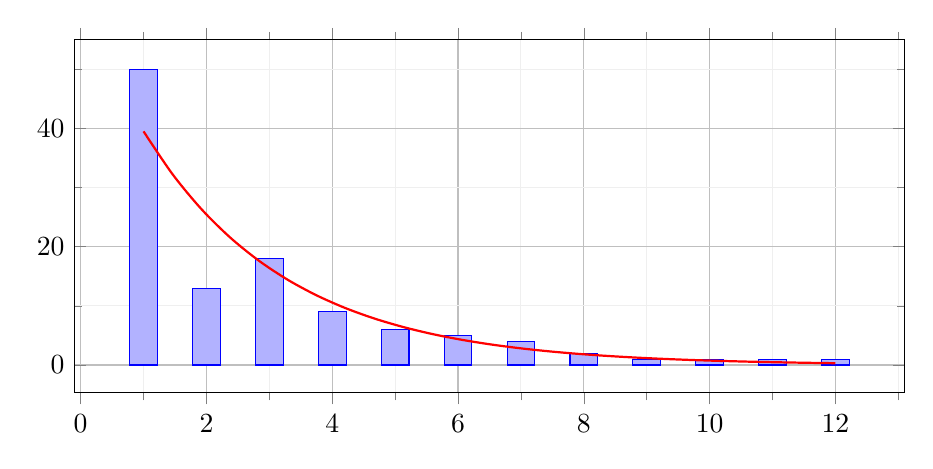
\begin{tikzpicture}
					\begin{axis} [
							ybar,
							grid = both,
							minor tick num = 1,
							major grid style = {lightgray},
							minor grid style = {lightgray!25},
							width = \textwidth,
							height = 0.5\textwidth
						]
						\addplot coordinates{
								(1 ,50)
								(2 ,13)
								(3 ,18)
								(4 ,9)
								(5 ,6)
								(6 ,5)
								(7 ,4)
								(8 ,2)
								(9 ,1)
								(10,1)
								(11,1)
								(12,1)
							};
						\addplot [
							domain = 1:12,
							smooth,
							thick,
							red,
						] {111*0.355769231*(1-0.355769231)^(x-1)};
					\end{axis}
				\end{tikzpicture}
			\end{center}
		\end{solution}
	\end{parts}

	% \newpage

	\question Consider an i.i.d. sample of random variables with Laplacian density function
	\[f(x|\sigma)=\frac{1}{2\sigma}\exp{\left(-\frac{|x|}{\sigma}\right)}\]

	\begin{parts}
		\part Find the method of moments estimate of \(\sigma\).

		\begin{solution}
			The pdf of the Laplacian distribution can be written piece-wise as,
			\[
				f(x|\sigma)=\begin{cases}
					\frac{1}{2\sigma}\exp{\left(-\frac{x}{\sigma}\right)} & x \ge 0 \\
					\frac{1}{2\sigma}\exp{\left(\frac{x}{\sigma}\right)}  & x < 0
				\end{cases}
			\]
			The moment generating function of the Laplacian distribution is,
			\begin{align*}
				M_{X}(t)= & \operatorname{E}\left[e^{tx}\right]                                                                                                                                                 \\
				=         & \int_{-\infty}^{\infty} e^{tx}\frac{1}{2\sigma}\exp{\left(-\frac{|x|}{\sigma}\right)}\mathrm{d} x                                                                                   \\
				=         & \frac{1}{2\sigma}\int_{0}^{\infty} e^{tx}\exp{\left(-\frac{x}{\sigma}\right)}\mathrm{d} x+\frac{1}{2\sigma}\int_{-\infty}^{0} e^{tx}\exp{\left(\frac{x}{\sigma}\right)}\mathrm{d} x \\
				=         & \frac{1}{2\sigma}\int_{0}^{\infty} e^{\left(t-\frac{1}{\sigma}\right)x}\mathrm{d} x+\frac{1}{2\sigma}\int_{-\infty}^{0} e^{\left(t+\frac{1}{\sigma}\right)x}\mathrm{d} x            \\
				=         & \frac{1}{2\sigma}\int_{0}^{\infty} e^{-\left(-t+\frac{1}{\sigma}\right)x}\mathrm{d} x+\frac{1}{2\sigma}\int_{0}^{\infty} e^{-\left(t+\frac{1}{\sigma}\right)x}\mathrm{d} x          \\
				=         & \frac{1}{2\sigma}\frac{1}{-t+\frac{1}{\sigma}}+\frac{1}{2\sigma}\frac{1}{t+\frac{1}{\sigma}}                                                                                        \\
				=         & \frac{1}{1-t^2\sigma^2}
			\end{align*}

			\(n\)th moment would be,

			\begin{align*}
				\mu_{n} & =\partial^{n}_{t}M_{X}(t)\big|_{t=0}                                                                                                                                                       \\
				        & =\frac{\partial^{n}}{\partial t^{n}}\left(\frac{1}{2\sigma}\frac{1}{t+\frac{1}{\sigma}}-\frac{1}{2\sigma}\frac{1}{t-\frac{1}{\sigma}}\right)\bigg|_{t=0}                                   \\
				        & =\frac{1}{2\sigma}\frac{\partial^{n}}{\partial t^{n}}\frac{1}{t+\frac{1}{\sigma}}\bigg|_{t=0}-\frac{1}{2\sigma}\frac{\partial^{n}}{\partial t^{n}}\frac{1}{t-\frac{1}{\sigma}}\bigg|_{t=0} \\
				        & =\frac{1}{2\sigma}\frac{(-1)^{n}n!}{\left(t+\frac{1}{\sigma}\right)^{n+1}}\bigg|_{t=0}-\frac{1}{2\sigma}\frac{(-1)^{n}n!}{\left(t-\frac{1}{\sigma}\right)^{n+1}}\bigg|_{t=0}               \\
				        & =\frac{n!\sigma^{n}}{2}((-1)^{n}+1)                                                                                                                                                        \\
			\end{align*}
			The first moments would be,
			\[\mu_{1} = 0 \qquad \mu_{2} = 2\sigma^{2}\]
			For \(N\) i.i.d. samples of the Laplacian distribution, the estimation of \(\sigma\) would be,
			\[\hat{\sigma} =\sqrt{\frac{\hat{\mu_{2}}}{2}} =\sqrt{\frac{\frac{1}{N}\sum_{i=1}^{N}x_{i}^{2}}{2}} = \sqrt{\frac{1}{2N}\sum_{i=1}^{N}x_{i}^{2}}\]
		\end{solution}

		\part Find the maximum likelihood estimate of \(\sigma\).

		\begin{solution}
			The log likelihood function of Laplacian distribution is,
			\begin{align*}
				l(\sigma) & =\log \left(\prod_{i=1}^{N} f(x_{i}|\sigma)\right)                                            \\
				          & =\sum_{i=1}^{N} \log f(x_{i}|\sigma)                                                          \\
				          & =\sum_{i=1}^{N} \log \left(\frac{1}{2\sigma}\exp{\left(-\frac{|x_{i}|}{\sigma}\right)}\right) \\
				          & =\sum_{i=1}^{N} \left(-\log{(2\sigma)}-\frac{|x_{i}|}{\sigma}\right)                          \\
				          & =-\frac{N}{2}\log{(2\sigma)}-\frac{1}{\sigma}\sum_{i=1}^{N}|x_{i}|
			\end{align*}
			The first derivative of the log likelihood function with respect to \(\sigma\) would be,
			\begin{align*}
				\frac{\partial l(\sigma)}{\partial \sigma} & =-\frac{N}{2\sigma}+\frac{1}{\sigma^{2}}\sum_{i=1}^{N}|x_{i}| \\
				\frac{\partial l(\sigma)}{\partial \sigma} & =0                                                            \\
				\implies \hat{\sigma}                      & =\frac{2}{N}\sum_{i=1}^{N}|x_{i}|
			\end{align*}
		\end{solution}
	\end{parts}

	% \newpage

	\question Suppose that \(X_{1},X_{2},\cdots,X_{25}\) are i.i.d. \(\mathcal{N}(\mu,\sigma^{2})\), where \(\mu=0\) and \(\sigma=10\). Plot the sampling distribution of \(\bar{X}\) and \(\hat{\sigma^{2}}\).

	\begin{solution}
		I used the following code to generate the 25 random samples from \(\mathcal{N}(0,100)\) and the distribution is ploted below it. Note that the code include the calculation of \(\bar{X}\) and \(\hat{\sigma^{2}}\) and also the plot of the sample distribution, but the distibution plot shown below is made using tikzpicture module of \LaTeX.
		\lstinputlisting[language=Python]{4.py}


		\begin{center}
			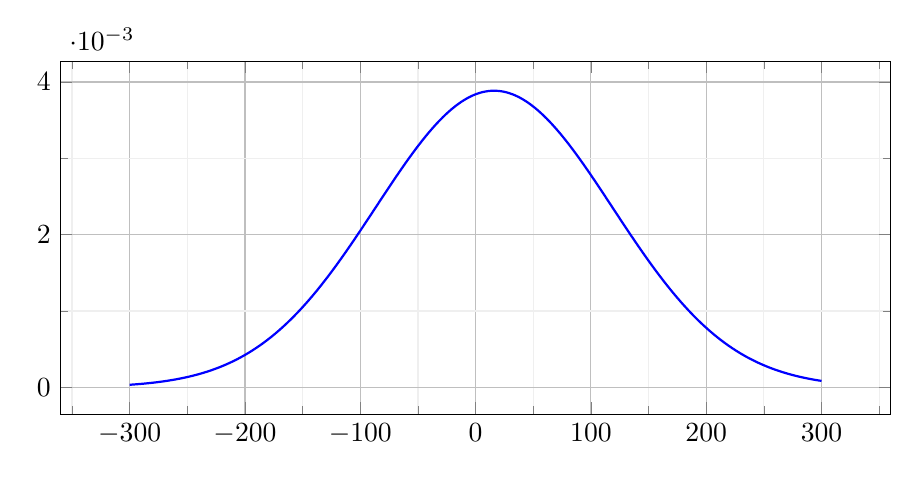
\begin{tikzpicture}
				\begin{axis} [
						grid = both,
						minor tick num = 1,
						major grid style = {lightgray},
						minor grid style = {lightgray!25},
						width = \textwidth,
						height = 0.5\textwidth
					]
					\addplot[
						domain = -300:300,
						samples = 1000,
						smooth,
						thick,
						blue,
					] {1/sqrt(2*pi*10543.220623706291)*exp(-1/2*(x-15.98254852780848)^2/10543.220623706291)};
				\end{axis}
			\end{tikzpicture}
		\end{center}
	\end{solution}

	% \newpage

	\question The following 16 numbers came from normal random number generator on a computer:
	\[\begin{array}{ccccccccc}
			5.3299 & 4.2537 & 3.1502 & 3.7032 & 1.6070 & 6.3923 & 3.1181 & 6.5941 \\
			3.5281 & 4.7433 & 0.1077 & 1.5977 & 5.4920 & 1.7220 & 4.1547 & 2.2799
		\end{array}\]

	\begin{parts}
		\part What would you guess the mean and variance (\(\mu\) and \(\sigma^{2}\)) of the generating normal distribution were?

		\begin{solution}
			The estimated mean of the distibution from where the numbers came is.
			\[\hat\mu=\frac{5.3299 + 4.2537 + \cdots + 2.2799}{16}=\frac{57.7739}{16}=3.61\]
			and the variance would be,
			\[\hat{\sigma^{2}}=\frac{(5.3299-3.61086875)^{2} + \cdots + (2.2799-3.61086875)^{2}}{16}=3.20\]
			\[s^{2}=3.413\]
		\end{solution}

		\part Give 90\%, 95\%, and 99\% confidence intervals for \(\mu\) and \(\sigma^{2}\).

		\begin{solution}
			We know that the confidence interval of \(\mu\) for \(100(1-\alpha)\%\) success rate is given by,
			\[\hat{\mu}-\hat{\sigma}\operatorname{z}\left(\frac{\alpha}{2}\right)\le\mu\le\hat{\mu}+\hat{\sigma}\operatorname{z}\left(\frac{\alpha}{2}\right)\]
			\[\implies 3.61-3.20\operatorname{z}\left(\frac{\alpha}{2}\right)\le\mu\le 3.61+3.20\operatorname{z}\left(\frac{\alpha}{2}\right)\]
			for \(\alpha = 0.10, 0.05, 0.01\) the confidence interval is,
			\begin{align*}
				3.61-3.20(1.645)\le \mu\le 3.61+3.20(1.645) & \implies -1.654 \le \mu\le 8.874    \\
				3.61-3.20(1.960)\le \mu\le 3.61+3.20(1.960) & \implies -2.662 \le \mu\le 9.882    \\
				3.61-3.20(2.576)\le \mu\le 3.61+3.20(2.576) & \implies -4.6332 \le \mu\le 11.8532
			\end{align*}
			We also know that the confidence interval of \(\sigma\) for \(100(1-\alpha)\%\) success rate is given by,
			\[\frac{(n-1)s^{2}}{\chi_{\alpha/2,n-1}}\le \sigma^{2} \le\frac{(n-1)s^{2}}{\chi_{1-\alpha/2,n-1}}\]
			for \(\alpha = 0.10, 0.05, 0.01\) the confidence interval is,
			\begin{align*}
				\frac{51.195}{\chi^{2}_{0.05,15}}\le \sigma^{2} \le\frac{51.195}{\chi^{2}_{0.95,15}}   & \implies 2.0481 \le \sigma^{2} \le 7.0508 \\
				\frac{51.195}{\chi^{2}_{0.025,15}}\le \sigma^{2} \le\frac{51.195}{\chi^{2}_{0.975,15}} & \implies 1.8624\le \sigma^{2} \le 8.1754  \\
				\frac{51.195}{\chi^{2}_{0.005,15}}\le \sigma^{2} \le\frac{51.195}{\chi^{2}_{0.995,15}} & \implies 1.5608\le \sigma^{2} \le 11.1272
			\end{align*}
		\end{solution}

		\part Give 90\%, 95\%, and 99\% confidence intervals for \(\sigma\).

		\begin{solution}
			\begin{align*}
				\alpha = 0.1   & \implies 1.4311 \le \sigma \le 2.6553 \\
				\alpha = 0.05  & \implies 1.3647 \le \sigma \le 2.8593 \\
				\alpha = 0.001 & \implies 1.2493 \le \sigma \le 3.3357
			\end{align*}
		\end{solution}

		% \part How much larger a sample do you think you would need to halve the length of the confidence interval for \(\mu\)?

		% \begin{solution}

		% \end{solution}
	\end{parts}

	% \newpage

	\question The Weibull distribution is defined in terms of CDF as follows:
	\[F(x)=1-e^{-\left(\frac{x}{\alpha}\right)^{\beta}},x\ge 0,\alpha>0,\beta>0\]

	\begin{parts}
		\part Generate Weibull distributed random numbers for given values of \(\alpha\) and \(\beta\) (using some existing tool).

		\begin{solution}

			I used the following code to generate the random numbers from Weibull distribution with \(\alpha=3\) and \(\beta=2\).
			\lstinputlisting[language=Python]{6.py}
			Following are the first 100 random numbers generated by one of the execution of the program.
			\begin{equation*}
				\begin{array}{cccccccccccccccccccc}
					2 & 3 & 1 & 2 & 5 & 3 & 3 & 3 & 3 & 3 & 1 & 1 & 3 & 1 & 2 & 4 & 3 & 2 & 3 & 5 \\
					1 & 1 & 3 & 2 & 3 & 3 & 0 & 1 & 6 & 1 & 1 & 2 & 0 & 4 & 3 & 3 & 1 & 3 & 1 & 4 \\
					2 & 4 & 5 & 4 & 3 & 1 & 2 & 4 & 2 & 2 & 4 & 6 & 1 & 1 & 1 & 4 & 6 & 0 & 4 & 4 \\
					2 & 6 & 5 & 2 & 3 & 4 & 3 & 1 & 4 & 4 & 1 & 1 & 2 & 1 & 2 & 1 & 1 & 3 & 1 & 2 \\
					2 & 1 & 3 & 1 & 1 & 1 & 1 & 3 & 2 & 2 & 3 & 4 & 4 & 0 & 6 & 3 & 2 & 3 & 5 & 5
				\end{array}
			\end{equation*}
		\end{solution}

		% \newpage

		\part Obtain the histogram of generated random numbers; normalize it and compare with true expression of PDF (they should be very close to each other).

		\begin{solution}
			\begin{center}
				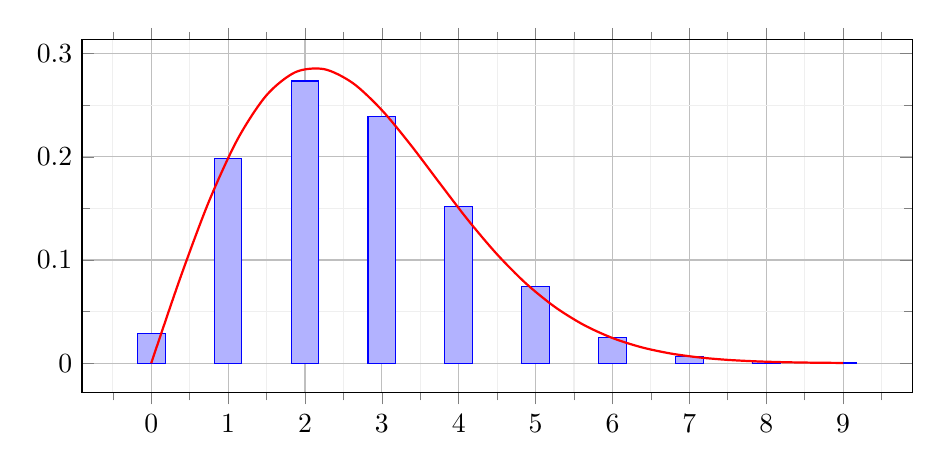
\begin{tikzpicture}
					\begin{axis} [
							ybar,
							grid = both,
							minor tick num = 1,
							major grid style = {lightgray},
							minor grid style = {lightgray!25},
							width = \textwidth,
							height = 0.5\textwidth
						]
						\addplot coordinates{
								(2, 0.2734)
								(1, 0.1981)
								(3, 0.2393)
								(4, 0.1522)
								(6, 0.025)
								(7, 0.0068)
								(5, 0.0742)
								(0, 0.0289)
								(8, 0.0017)
								(9, 0.0004)
							};
						\addplot [
							domain = 0:9,
							smooth,
							thick,
							red
						] {2/x*(x/3)^2*exp(-(x/3)^2) };
					\end{axis}
				\end{tikzpicture}
			\end{center}
		\end{solution}

		\part Write a (recursive or iterative) computer code to compute the estimate the values of \(\alpha\) and \(\beta\) using expressions (1) and (2), respectively, for the data generated in step 1 (above). Note: For large enough data, the estimated and true values must be very close to each other.

		\begin{solution}
			The expressions given in the question are:
			\[\hat{\alpha} = \left(\frac{1}{n}\sum_{i=1}^{n}x_{i}^{\hat{\beta}}\right)^{\frac{1}{\hat{\beta}}}\]
			\[\hat\beta\left(\frac{\sum_{i=1}^{n}x_{i}^{\hat\beta}\log{x_{i}}}{\sum_{i=1}^{n}x_{i}^{\hat\beta}}-\frac{1}{n}\sum_{i=1}^{n}\log{x_{i}}\right)=1\]
			We will first numerically approximate \(\hat\beta\) because it only depends on \(x_{i}\). We will then use this value to compute \(\hat{\alpha}\). Now let,
			\[f(\hat\beta) = \hat\beta\left(\frac{\sum_{i=1}^{n}x_{i}^{\hat\beta}\log{x_{i}}}{\sum_{i=1}^{n}x_{i}^{\hat\beta}}-\frac{1}{n}\sum_{i=1}^{n}\log{x_{i}}\right)-1\]
			For a very small step \(\delta\), the derivative of \(f\) can be approximated as,
			\[f'(\beta)\approx\frac{f(\beta+\delta)-f(\beta)}{\delta}\]
			For our initial guess \(\beta_{0}\), the Newton-Raphson method can be used to find the root of \(f\) as follows:
			\[\beta_{k+1}=\beta_{k}-\frac{f(\beta_{k})}{f'(\beta_{k})}\]
			The following code approximates the value of \(\hat\beta\) and \(\hat\alpha\) using the above method.
			\lstinputlisting[language=Python]{6b.py}
			Output from one execution of the above code. (Note: each time one would get a different output.)
			\begin{verbatim}
beta = 2.9846029948504746
error in the value of beta = 0.513 %
alpha = 1.9943804254801567
error in the value of alpha = 0.281 %
            \end{verbatim}
		\end{solution}
	\end{parts}
\end{questions}

\end{document}